\chapter{\textbf{Capitulo III: Análisis}}

\section{Análisis Preliminar}

Para el cálculo de la nómina, actualmente se cuenta con un dispositivo lector de huella digital en el cual los colaboradores registran su ingreso y salida de su jornada laboral. Esta información es extraída manualmente por el personal administrativo y luego procesada en hojas de cálculo, lo cual representa una tarea operativa repetitiva, propensa a errores humanos y sin integración con otros procesos internos.

Aunque existe un mecanismo básico de registro de jornada, la ausencia de un sistema que centralice y automatice el procesamiento de dicha información genera cuellos de botella en actividades como la emisión de reportes, la gestión de eventos laborales (vacaciones, incapacidades, permisos especiales), y la elaboración de comprobantes de pago.

Este análisis evidencia la necesidad de optimizar el flujo de información ya disponible en el entorno organizacional, de modo que pueda ser aprovechada de forma estructurada y confiable mediante una solución tecnológica que integre las funcionalidades necesarias para mejorar la eficiencia y la trazabilidad del proceso.

\subsection{Gestión de Riesgos}

La gestión de riesgos es un proceso esencial dentro del desarrollo del sistema web de gestión de nómina para Café y Vivero Verde Pradera. Su propósito es identificar, analizar y mitigar los eventos que puedan afectar el cumplimiento de los objetivos del proyecto, tanto en el ámbito técnico como en el administrativo.
Durante la fase actual, se han presentado desafíos reales relacionados con la instalación de la base de datos, la conexión con el reloj marcador y la falta de documentación sobre el cálculo de nómina por parte de la empresa, los cuales se incluyen dentro de los riesgos evaluados.

\subsubsection*{Identificación de Riesgos}

Durante el análisis y ejecución del proyecto, se identificaron los siguientes riesgos potenciales:

\begin{itemize}
	\item \textbf{Retrasos en la planificación:} Posibles demoras en la entrega de hitos o tareas clave que afecten el cronograma general del proyecto.
	\item \textbf{Falta de definición de requerimientos:} Cambios frecuentes o ausencia de información precisa sobre los requisitos funcionales y no funcionales, generando reprocesos.
	\item \textbf{Problemas de comunicación con la empresa:} Dificultades para concretar reuniones o recibir la documentación necesaria para avanzar en los módulos de cálculo de nómina.
	\item \textbf{Retrasos en la instalación de la base de datos:} Dificultades técnicas o falta de acceso al servidor de la empresa que impiden continuar con las pruebas e integración del sistema.
	\item \textbf{Errores en la integración del reloj marcador:} Problemas para conectar el sistema con el dispositivo de marcación, afectando el registro automático de asistencias.
	\item \textbf{Capacitación insuficiente del equipo:} Limitaciones técnicas o desconocimiento de herramientas clave que ralentizan el desarrollo o la configuración del sistema.
	\item \textbf{Asignación inadecuada de recursos:} Distribución deficiente del tiempo, personal o herramientas, afectando la eficiencia general del proyecto.
	\item \textbf{Problemas en el control de versiones:} Conflictos o pérdida de integridad del código debido a una gestión inadecuada del repositorio.
	\item \textbf{Falta de pruebas tempranas:} Postergación de pruebas unitarias o de integración, impidiendo detectar errores críticos de manera oportuna.
	\item \textbf{Limitaciones presupuestarias durante el desarrollo:} Falta de fondos para cubrir recursos técnicos, licencias o servicios en la nube necesarios para la implementación.
\end{itemize}

\subsubsection*{Matriz de Probabilidad por Impacto (escala 3x3)}

Para esta evaluación se utiliza una escala simplificada de 1 a 3 tanto para la probabilidad como para la gravedad (impacto), donde:

\begin{itemize}
	\item \textbf{Probabilidad:}
	      \begin{itemize}
		      \item 1 = Baja
		      \item 2 = Media
		      \item 3 = Alta
	      \end{itemize}
	\item \textbf{Gravedad (Impacto):}
	      \begin{itemize}
		      \item 1 = Leve
		      \item 2 = Serio
		      \item 3 = Muy serio
	      \end{itemize}
\end{itemize}

El nivel de riesgo (\textit{N}) se obtiene multiplicando ambos factores. Los valores se clasifican según la siguiente escala:


\begin{center}
	\begin{tikzpicture}
		% Colores
		\definecolor{lowrisk}{RGB}{144,238,144}      % Verde
		\definecolor{medrisk}{RGB}{255,255,153}      % Amarillo
		\definecolor{elevrisk}{RGB}{255,204,153}     % Naranja suave
		\definecolor{highrisk}{RGB}{255,0,0}         % Rojo

		% Matriz 3x3 (Probabilidad: columnas 1..3; Gravedad: filas 1..3, de abajo hacia arriba)
		% Fila Gravedad=3 (arriba): valores 3,6,9  -> Amarillo, Naranja, Rojo
		\matrix[matrix of nodes,
			nodes={minimum height=1cm,minimum width=1.2cm,draw,anchor=center},
			row sep=-\pgflinewidth,column sep=-\pgflinewidth] (m) {
			\node[fill=medrisk] {3}; & \node[fill=elevrisk] {6}; & \node[fill=highrisk] {9}; \\
			\node[fill=lowrisk] {2}; & \node[fill=medrisk] {4};  & \node[fill=elevrisk] {6}; \\
			\node[fill=lowrisk] {1}; & \node[fill=lowrisk] {2};  & \node[fill=medrisk] {3};  \\
		};

		% Etiquetas de ejes
		\node[rotate=90] at ([xshift=-1.2cm]m.west) {\textbf{Gravedad}};
		\node at ([yshift=1.2cm]m.north) {\textbf{Probabilidad}};

	\end{tikzpicture}
\end{center}


\newpage

\begin{table}[h!]
	\centering
	\begin{tabular}{|p{6cm}|c|c|c|}
		\hline
		\textbf{Riesgo}                                    & \textbf{Prob. (1–3)} & \textbf{Gravedad (1–3)} & \textbf{Nivel (N)} \\ \hline
		Retrasos en la planificación                       & 2                    & 2                       & 4 (Medio)          \\ \hline
		Falta de definición de requerimientos              & 1                    & 3                       & 3 (Bajo)           \\ \hline
		Problemas de comunicación con la empresa           & 3                    & 2                       & 6 (Crtico)         \\ \hline
		Retrasos en la instalación de la base de datos     & 3                    & 3                       & 9 (Crítico)        \\ \hline
		Errores en la integración del reloj marcador       & 3                    & 3                       & 9 (Crítico)        \\ \hline
		Capacitación insuficiente del equipo               & 2                    & 2                       & 4 (Medio)          \\ \hline
		Asignación inadecuada de recursos                  & 2                    & 2                       & 4 (Medio)          \\ \hline
		Problemas en el control de versiones               & 2                    & 1                       & 2 (Bajo)           \\ \hline
		Falta de pruebas tempranas                         & 3                    & 2                       & 6 (Medio)          \\ \hline
		Limitaciones presupuestarias durante el desarrollo & 1                    & 1                       & 1 (Bajo)           \\ \hline
	\end{tabular}
	\caption{Matriz de probabilidad por impacto (escala 3x3) del proyecto VP-Planilla}
	\label{tab:matriz_prob_impacto_3x3}
\end{table}

\subsubsection*{Plan de Tratamiento de Riesgos}

Con base en la matriz de probabilidad e impacto (escala 3×3), se definieron las estrategias preventivas y correctivas necesarias para reducir los efectos de los riesgos identificados en el proyecto VP-Planilla. Los riesgos se agrupan según su nivel de severidad: Crítico, Medio o Bajo.

\paragraph{Riesgos Críticos}
\begin{itemize}
	\item \textbf{Problemas de comunicación con la empresa (N = 6):}
	      La falta de coordinación y retrasos en las respuestas pueden afectar la validación de requerimientos y las decisiones técnicas.
	      \textit{Acciones:} establecer un calendario fijo de reuniones semanales, utilizar canales formales de comunicación (correo institucional o grupo de trabajo) y registrar actas con los acuerdos alcanzados.

	\item \textbf{Retrasos en la instalación de la base de datos (N = 9):}
	      La imposibilidad de instalar la base de datos en el servidor de la empresa ha limitado las pruebas de integración.
	      \textit{Acciones:} mantener una base temporal en Docker o Neon.tech mientras se gestiona el acceso al servidor de la empresa; documentar el proceso de instalación para replicarlo en producción.

	\item \textbf{Retraso en la integración del reloj marcador (N = 6):}
	      Los problemas de conexión con el dispositivo dificultan el registro automático de asistencias.
	      \textit{Acciones:} simular los datos de marcación mientras se obtiene acceso al reloj físico; desarrollar rutinas de importación y exportación mediante archivos CSV o API.
\end{itemize}

\paragraph{Riesgos Medios}
\begin{itemize}
	\item \textbf{Retrasos en la planificación (N = 4):}
	      Las entregas podrían no cumplirse conforme al cronograma propuesto.
	      \textit{Acciones:} dividir el trabajo en entregas semanales, asignar responsables y usar herramientas de seguimiento (Trello, GitHub Projects) para monitorear avances.

	\item \textbf{Capacitación insuficiente del equipo (N = 4):}
	      Algunas limitaciones técnicas pueden retrasar tareas específicas del desarrollo.
	      \textit{Acciones:} realizar talleres internos sobre Docker, PostgreSQL y control de versiones; generar guías prácticas para el equipo.

	\item \textbf{Asignación inadecuada de recursos (N = 4):}
	      Una mala distribución del tiempo o tareas puede disminuir la eficiencia general.
	      \textit{Acciones:} revisar la carga de trabajo, redistribuir responsabilidades y priorizar las tareas más críticas.

	\item \textbf{Falta de pruebas tempranas (N = 6):}
	      La ausencia de validaciones en etapas iniciales puede generar errores en fases avanzadas.
	      \textit{Acciones:} planificar pruebas unitarias y de integración semanales; revisar los resultados antes de cada entrega parcial.
\end{itemize}

\paragraph{Riesgos Bajos}
\begin{itemize}
	\item \textbf{Falta de definición de requerimientos (N = 3):}
	      A pesar de tener bajo riesgo, una definición incompleta puede generar pequeños reprocesos.
	      \textit{Acciones:} documentar los requerimientos mínimos viables y validarlos formalmente con la empresa antes de avanzar en el desarrollo.

	\item \textbf{Problemas en el control de versiones (N = 2):}
	      Podrían surgir conflictos en el código por fusiones incorrectas o falta de coordinación.
	      \textit{Acciones:} definir ramas de trabajo (\textit{main}, \textit{dev}, \textit{feature}), realizar revisiones de código y establecer políticas de commits.

	\item \textbf{Limitaciones presupuestarias durante el desarrollo (N = 1):}
	      Las limitaciones económicas actuales no representan un riesgo significativo, pero pueden afectar adquisiciones puntuales.
	      \textit{Acciones:} continuar utilizando herramientas de código abierto (PostgreSQL, GitHub, Docker) y optimizar los recursos disponibles en el entorno de desarrollo.
\end{itemize}

\paragraph{Síntesis General}
Los riesgos críticos se concentran en la comunicación con la empresa y en aspectos técnicos como la base de datos y el reloj marcador.
Los riesgos medios corresponden a la planificación, capacitación y pruebas internas, mientras que los bajos se relacionan con factores administrativos o de soporte.
El monitoreo constante y la documentación de cada avance permitirán reducir la probabilidad de retrasos y asegurar la estabilidad del sistema VP-Planilla durante su desarrollo.


\newpage
\subsection{Estudio de factibilidad y Gestión de Riesgo}

\subsubsection{Factibilidad Operativa}

\begin{itemize}
	\item \textbf{Conocimiento de los desarrolladores:} Los desarrolladores del sistema son estudiantes avanzados de Ingeniería en Sistemas, con experiencia en desarrollo web, bases de datos y metodologías ágiles, lo que garantiza una correcta implementación del proyecto.

	\item \textbf{Habilidad de los usuarios:} El sistema está orientado al personal administrativo de la empresa, quienes ya realizan los procesos manuales y tienen el conocimiento necesario para adaptarse al uso de un sistema digital. Se planea además incluir una etapa de capacitación.

	\item \textbf{Disponibilidad de horarios:} Tanto el equipo de desarrollo como el personal administrativo disponen de horarios establecidos para reuniones de revisión, pruebas e implementación.

	\item \textbf{Mantenimiento del software:} El sistema será documentado técnicamente y se mantendrá en un repositorio GitHub, lo cual facilitará futuras mejoras, corrección de errores y mantenimiento general.
\end{itemize}

\textbf{Conclusión:} Existe una alta viabilidad operativa para implementar el sistema, debido a la disposición de los usuarios, la experiencia del equipo desarrollador y la estructura de apoyo brindada por la empresa.

\subsubsection{Factibilidad Técnica}

\begin{itemize}
	\item \textbf{Especificación de Hardware y Software:} El sistema funcionará sobre servidores con al menos 4~GB de RAM y 20~GB de almacenamiento. Los usuarios accederán desde navegadores modernos como Chrome o Edge.

	\item \textbf{Infraestructura de redes:} La empresa cuenta con conexión a internet estable, lo cual permite que el sistema funcione correctamente en modalidad web. Inicialmente, el sistema será hospedado en un servidor local dentro de las instalaciones de la empresa, aunque se deja abierta la posibilidad de migración futura a un servicio en la nube si las necesidades operativas así lo requieren.

	\item \textbf{Herramientas de desarrollo:} Se utilizarán herramientas como Visual Studio Code, GitHub, PostgreSQL, Next.js, Node.js y Prisma ORM, todas gratuitas y ampliamente documentadas.

	\item \textbf{Plataformas de desarrollo:} El sistema será construido como una aplicación web, compatible con sistemas operativos modernos. El backend correrá en Node.js y el frontend en Next.js con TypeScript.
\end{itemize}

\textbf{Conclusión:} El proyecto es técnicamente viable gracias a la disponibilidad de herramientas, infraestructura básica y conocimientos del equipo para implementar la solución sin depender de tecnologías costosas o inaccesibles.

\subsubsection{Factibilidad Económica}

La factibilidad económica busca determinar la viabilidad del proyecto desde el punto de vista financiero, considerando los costos asociados al desarrollo e implementación del sistema de nómina.
Dado que se trata de un proyecto académico, la mayor parte de los recursos corresponden al tiempo de trabajo y al uso de software libre, con pocos gastos directos.

\begin{itemize}
	\item \textbf{Costos de desarrollo:} El proyecto no implica contratación de personal externo, ya que el desarrollo será realizado por estudiantes de Ingeniería en Sistemas.
	      Se estima un valor simbólico por la dedicación académica de 160 horas por estudiante, con un costo referencial de ₡3.000,00 por hora, equivalente a ₡480.000,00 por estudiante.

	\item \textbf{Costos de capital humano:} Para un equipo de dos desarrolladores, el costo simbólico total asciende a ₡960.000,00.

	\item \textbf{Adquisición de hardware:} La empresa adquirirá un \textit{reloj marcador biométrico} nuevo, con un costo de ₡201.705,00 (precio estimado de mercado en Costa Rica).

	\item \textbf{Servidor local:} La empresa cuenta con una computadora que puede funcionar como servidor.
	      En caso de renovación o sustitución, se estima un costo de ₡480.000,00 para un equipo de gama media-alta con procesador Intel i5/AMD Ryzen 5, 16~GB de RAM y SSD de 512~GB (según precios consultados en ExtremeTech Costa Rica, octubre 2025).

	\item \textbf{Software y herramientas:} No se requieren licencias de pago, ya que se utilizarán soluciones de código abierto como PostgreSQL, Node.js, Next.js, Prisma ORM y GitHub.

	\item \textbf{Cargos administrativos:} El tiempo del personal administrativo destinado a validaciones se considera parte de las operaciones normales de la empresa, por lo tanto, no genera costos adicionales.
\end{itemize}

\begin{table}[h!]
	\centering
	\begin{tabular}{|p{7cm}|r|}
		\hline
		\textbf{Rubro}                                  & \textbf{Costo (₡)}        \\ \hline
		Valor simbólico del desarrollo (2 estudiantes)  & \col960.000,00            \\ \hline
		Compra de reloj marcador biométrico             & \col201.705,00            \\ \hline
		Presupuesto de servidor (en caso de renovación) & \col480.000,00            \\ \hline
		Software y licencias (código abierto)           & \col0,00                  \\ \hline
		Cargos administrativos internos                 & \col0,00                  \\ \hline
		\textbf{Total estimado del proyecto}            & \textbf{\col1.641.705,00} \\ \hline
	\end{tabular}
	\caption{Desglose de costos estimados del proyecto VP-Planilla}
	\label{tab:costos_vp_planilla}
\end{table}

\textbf{Conclusión:}
El sistema de gestión de nómina para Café y Vivero Verde Pradera presenta una alta viabilidad económica.
Su inversión principal corresponde al tiempo de desarrollo de los estudiantes y la compra de un reloj marcador, con la posibilidad de renovación del servidor en el futuro.
El uso de software libre y recursos existentes permite mantener el costo total en aproximadamente ₡1.641.705,00, lo que convierte al proyecto en una solución accesible, sostenible y de alto impacto para la gestión administrativa de la empresa.

\subsection{Ciclo de vida}

Para el desarrollo del sistema de gestión de nóminas para Café y Vivero Verde Pradera se aplicará un enfoque ágil, utilizando la metodología \textbf{Scrum}, complementada con un modelo de \textbf{Desarrollo Incremental}. El proceso se organizará en ocho sprints consecutivos, cada uno con una duración estimada de dos semanas.

Cada sprint tiene como objetivo generar un incremento funcional del sistema, es decir, una parte del software que puede ser evaluada y validada internamente. Sin embargo, estas versiones no se instalarán en un entorno productivo al finalizar cada sprint. La instalación oficial del sistema completo se realizará al final del último sprint, tras pasar por una fase integral de pruebas y validaciones.

Durante cada sprint se realizará una etapa de revisión y retroalimentación (\textit{Feedback}), que permitirá hacer ajustes continuos y asegurar que las funcionalidades desarrolladas cumplan con los requerimientos establecidos.


\begin{itemize}
	\item \textbf{Sprint 1: Setup del Proyecto} \\
	      Inicialización del entorno de desarrollo, configuración del repositorio GitHub y definición de la estructura base del sistema.

	\item \textbf{Sprint 2: Módulo de Login} \\
	      Desarrollo del sistema de autenticación de usuarios y control de acceso.

	\item \textbf{Sprint 3: Módulo de Interfaz de Usuario} \\
	      Implementación del diseño general del frontend y componentes base de navegación.

	\item \textbf{Sprint 4: Administración de Eventos Laborales} \\
	      Funcionalidad para registrar y gestionar vacaciones, incapacidades y permisos.

	\item \textbf{Sprint 5: Cálculo de Nóminas} \\
	      Implementación del motor de cálculo automático de salarios y deducciones.

	\item \textbf{Sprint 6: Generación de Reportes} \\
	      Emisión de reportes institucionales y comprobantes de pago para los empleados.

	\item \textbf{Sprint 7: Módulo de Seguridad} \\
	      Validaciones adicionales, cifrado de contraseñas, roles y permisos de usuario.

	\item \textbf{Sprint 8: Pruebas y Entrega} \\
	      Pruebas funcionales, validación con usuarios, documentación final y entrega del sistema.
\end{itemize}

\newpage

\subsection{Estructura de Desglose del Trabajo (EDT)}

La Estructura de Desglose del Trabajo (EDT) permite organizar el proyecto en fases y
tareas específicas de manera jerárquica. En este caso, se divide en cinco fases principales
que agrupan las actividades necesarias para el desarrollo del sistema de gestión de nóminas.
La siguiente figura representa gráficamente esta estructura, facilitando la planificación y el seguimiento del proyecto.

\begin{figure}[h!]
	\centering
	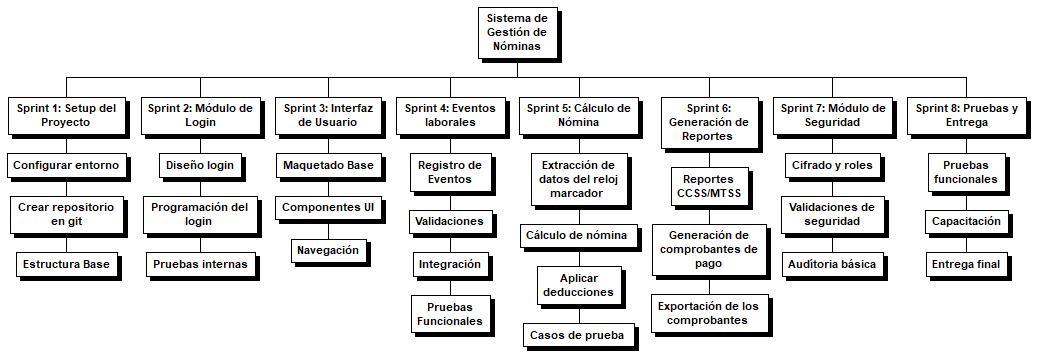
\includegraphics[width=1.0\textwidth]{media/WBS.png}
	\caption{Estructura de Desglose del Trabajo del Proyecto (EDT) basada en sprints}
	\label{fig:edt}
\end{figure}


\subsection*{Product Backlog}

Antes de desarrollar las historias de usuario, se construyó un \textbf{Product Backlog} con las funcionalidades principales del sistema. Este backlog funciona como una lista priorizada de los entregables que serán desarrollados a lo largo de los sprints definidos. Cada ítem representa una funcionalidad o módulo del sistema, estimado en complejidad y valor para el usuario final.

El backlog sirve como guía para la planificación iterativa del proyecto, y puede evolucionar conforme se obtenga retroalimentación durante las etapas de desarrollo.

\begin{itemize}
	\item Autenticación y control de acceso
	\item Registro de jornada laboral desde lector de huella
	\item Gestión de eventos laborales (vacaciones, incapacidades)
	\item Cálculo automático de nómina
	\item Generación de reportes institucionales
	\item Emisión de comprobantes de pago
	\item Módulo de administración de usuarios
	\item Seguridad y roles
	\item Capacitación y documentación
\end{itemize}

\subsection*{Historias de Usuario}

Las historias de usuario permiten capturar de manera sencilla y centrada en el usuario las funcionalidades esperadas del sistema de gestión de nóminas para Café y Vivero Verde Pradera. Estas historias han sido redactadas desde la perspectiva de los distintos tipos de usuarios del sistema (administradores, colaboradores y gerentes), con el fin de comprender sus necesidades, priorizar el desarrollo de funcionalidades y planificar el trabajo en sprints.

Cada historia incluye información clave como el usuario involucrado, la prioridad del requerimiento, el riesgo asociado, la iteración en que se desarrollará, la estimación de esfuerzo y una breve descripción del comportamiento esperado del sistema.

Estas historias se utilizarán como base para guiar el diseño, implementación y pruebas de cada funcionalidad a lo largo del desarrollo del proyecto.

\begin{table}[h]
	\centering
	\caption{Historia de Usuario HU-01}
	\begin{tabular}{|p{5cm}|p{9cm}|}
		\hline
		\textbf{Número:}                          & HU-01                           \\ \hline
		\textbf{Nombre:}                          & Gestión de usuarios del sistema \\ \hline
		\textbf{Usuario:}                         & Administrador                   \\ \hline
		\textbf{Modificación de Historia Número:} & Nueva                           \\ \hline
		\textbf{Prioridad en Negocio:}            & Alta                            \\ \hline
		\textbf{Riesgo en Desarrollo:}            & Medio                           \\ \hline
		\textbf{Iteración Asignada:}              & Sprint 2: Módulo de Login       \\ \hline
		\textbf{Puntos Estimados:}                & 5                               \\ \hline
		\textbf{Puntos Reales:}                   & --                              \\ \hline
		\textbf{Descripción:}                     &
		El sistema permitirá al administrador realizar operaciones CRUD (Crear, Leer, Actualizar, Eliminar) sobre los usuarios registrados.
		El administrador podrá:
		\begin{itemize}
			\item Crear nuevos usuarios ingresando nombre, correo y rol.
			\item Consultar la lista de usuarios registrados.
			\item Editar los datos de un usuario existente (excepto el ID).
			\item Eliminar usuarios en caso de salida de personal.
		\end{itemize}
		Las acciones estarán disponibles únicamente para usuarios con rol de Administrador autenticado. Todas las operaciones deben registrar trazabilidad en la bitácora del sistema.
		\\ \hline
		\textbf{Observaciones:}                   &
		El correo ingresado debe ser validado en formato y unicidad. No se podrá eliminar al usuario con sesión activa.
		Solo se permite modificar el rol o correo si el usuario está inactivo.
		El sistema debe confirmar cada operación antes de ejecutarla.
		\\ \hline
	\end{tabular}
\end{table}


\begin{table}[h]
	\centering
	\caption{Historia de Usuario HU-02}
	\begin{tabular}{|p{5cm}|p{9cm}|}
		\hline
		\textbf{Número:}                          & HU-02                                   \\ \hline
		\textbf{Nombre:}                          & Gestión de roles de usuario             \\ \hline
		\textbf{Usuario:}                         & Administrador                           \\ \hline
		\textbf{Modificación de Historia Número:} & Nueva                                   \\ \hline
		\textbf{Prioridad en Negocio:}            & Alta                                    \\ \hline
		\textbf{Riesgo en Desarrollo:}            & Bajo                                    \\ \hline
		\textbf{Iteración Asignada:}              & Sprint 3: Módulo de Interfaz de Usuario \\ \hline
		\textbf{Puntos Estimados:}                & 5                                       \\ \hline
		\textbf{Puntos Reales:}                   & --                                      \\ \hline
		\textbf{Descripción:}                     &
		El sistema permitirá al administrador realizar operaciones CRUD sobre los roles asignados a los usuarios. Estas operaciones incluyen:
		\begin{itemize}
			\item \textbf{Crear:} Definir nuevos roles dentro del sistema si se requiere extender la funcionalidad futura.
			\item \textbf{Leer:} Consultar el rol asignado a cada usuario.
			\item \textbf{Actualizar:} Modificar el rol de un usuario existente.
			\item \textbf{Eliminar:} Eliminar roles obsoletos, siempre que no estén asignados a usuarios activos.
		\end{itemize}
		El administrador podrá ingresar a la sección de gestión de roles, seleccionar un usuario, visualizar los roles disponibles y asignar o modificar el rol correspondiente. El sistema guardará los cambios y mostrará una confirmación.
		\\ \hline
		\textbf{Observaciones:}                   &
		Cada usuario solo puede tener un rol activo a la vez.
		No se permitirá eliminar un rol si está actualmente asignado a uno o más usuarios.
		La acción de cambio de rol debe registrarse en la bitácora del sistema.
		La asignación de roles debe estar protegida por validación de permisos del administrador.
		\\ \hline
	\end{tabular}
\end{table}


\begin{table}[h]
	\centering
	\caption{Historia de Usuario HU-03}
	\begin{tabular}{|p{5cm}|p{9cm}|}
		\hline
		\textbf{Número:}                          & HU-03                                         \\ \hline
		\textbf{Nombre:}                          & Entrega automática de comprobantes de pago    \\ \hline
		\textbf{Usuario:}                         & Colaborador                                   \\ \hline
		\textbf{Modificación de Historia Número:} & Actualización - acceso por correo electrónico \\ \hline
		\textbf{Prioridad en Negocio:}            & Media                                         \\ \hline
		\textbf{Riesgo en Desarrollo:}            & Bajo                                          \\ \hline
		\textbf{Iteración Asignada:}              & Sprint 5: Cálculo de Nóminas                  \\ \hline
		\textbf{Puntos Estimados:}                & 5                                             \\ \hline
		\textbf{Puntos Reales:}                   & --                                            \\ \hline
		\textbf{Descripción:}                     &
		El sistema enviará automáticamente al colaborador un comprobante de pago por correo electrónico cada vez que se procese una nómina. El comprobante incluirá el monto neto recibido, fecha del pago, deducciones y cualquier concepto adicional, como aguinaldo.

		El colaborador no accede al sistema. El correo de destino deberá haber sido previamente registrado por un administrador en su ficha de empleado.

		\textbf{CRUD:}
		\begin{itemize}
			\item \textbf{Crear:} El sistema crea el comprobante al procesar la nómina.
			\item \textbf{Leer:} No aplica para el colaborador. El sistema genera y envía automáticamente el comprobante.
			\item \textbf{Actualizar:} El administrador podrá corregir un comprobante si hay rectificación en la nómina.
			\item \textbf{Eliminar:} No se eliminan comprobantes. Si es necesario, se envía una versión corregida.
		\end{itemize}
		\\ \hline
		\textbf{Observaciones:}                   &
		Todo comprobante será enviado al correo proporcionado y validado por el colaborador al ser registrado. El contenido del correo será cifrado si la organización así lo define, y deberá cumplir con los lineamientos del Ministerio de Trabajo.
		\\ \hline
	\end{tabular}
\end{table}





\begin{table}[h]
	\centering
	\caption{Historia de Usuario HU-04}
	\begin{tabular}{|p{5cm}|p{10cm}|}
		\hline
		\textbf{Número:}                          & HU-04                                      \\ \hline
		\textbf{Nombre:}                          & Generación y gestión de reportes de nómina \\ \hline
		\textbf{Usuario:}                         & Gerente                                    \\ \hline
		\textbf{Modificación de Historia Número:} & Actualización - incluye aguinaldo          \\ \hline
		\textbf{Prioridad en Negocio:}            & Alta                                       \\ \hline
		\textbf{Riesgo en Desarrollo:}            & Alto                                       \\ \hline
		\textbf{Iteración Asignada:}              & Sprint 6: Generación de Reportes           \\ \hline
		\textbf{Puntos Estimados:}                & 5                                          \\ \hline
		\textbf{Puntos Reales:}                   & --                                         \\ \hline
		\textbf{Descripción:}                     &
		El sistema permitirá al gerente generar, visualizar y gestionar reportes de nómina. Desde el módulo correspondiente, el usuario podrá seleccionar el mes deseado y obtener un archivo PDF que incluya detalles de salarios brutos, deducciones, aportes patronales y salario neto total.

		En el mes de diciembre, el reporte incluirá una línea separada con el cálculo del aguinaldo de cada empleado, conforme a la normativa laboral vigente.

		Las operaciones CRUD asociadas a esta historia son:
		\begin{itemize}
			\item \textbf{Crear:} Generación de un nuevo reporte mensual al cierre de la nómina.
			\item \textbf{Leer:} Consultar reportes anteriores, filtrados por mes o año.
			\item \textbf{Actualizar:} Regenerar un reporte si se realizaron ajustes a la nómina.
			\item \textbf{Eliminar:} Borrar reportes bajo condiciones de auditoría (solo si no han sido firmados o validados).
		\end{itemize}
		Todos los reportes deberán conservar trazabilidad en la bitácora del sistema y permitir exportación a PDF.
		\\ \hline
		\textbf{Observaciones:}                   &
		Esta funcionalidad estará restringida exclusivamente a usuarios con rol de Gerente. El sistema debe validar la autenticación y el rol activo antes de permitir acceso. Todos los archivos generados deberán protegerse mediante encriptación y almacenamiento seguro. En el caso del aguinaldo, el sistema deberá asegurar que los datos provienen del cálculo realizado previamente, y mostrar el monto correspondiente de forma clara y diferenciada.
		\\ \hline
	\end{tabular}
\end{table}


\begin{table}[h]
	\centering
	\caption{Historia de Usuario HU-05}
	\begin{tabular}{|p{5cm}|p{9cm}|}
		\hline
		\textbf{Número:}                          & HU-05                                                                                                                                                                                                \\ \hline
		\textbf{Nombre:}                          & Registro de llegada y salida de jornada laboral                                                                                                                                                      \\ \hline
		\textbf{Usuario:}                         & Colaborador                                                                                                                                                                                          \\ \hline
		\textbf{Modificación de Historia Número:} & Nueva                                                                                                                                                                                                \\ \hline
		\textbf{Prioridad en Negocio:}            & Alta                                                                                                                                                                                                 \\ \hline
		\textbf{Riesgo en Desarrollo:}            & Medio                                                                                                                                                                                                \\ \hline
		\textbf{Iteración Asignada:}              & Sprint 4: Eventos Laborales                                                                                                                                                                          \\ \hline
		\textbf{Puntos Estimados:}                & 5                                                                                                                                                                                                    \\ \hline
		\textbf{Puntos Reales:}                   & --                                                                                                                                                                                                   \\ \hline
		\textbf{Descripción:}                     &
		El colaborador registrará su ingreso y salida mediante un lector de huella o interfaz web. El sistema almacenará la hora exacta, la fecha y el ID del usuario, generando un historial de asistencia consultable por los administradores.

		\textbf{CRUD:}
		\begin{itemize}
			\item \textbf{Crear:} Registro automático del ingreso y salida al marcar asistencia.
			\item \textbf{Leer:} Consulta de historial por parte de administradores o el mismo colaborador.
			\item \textbf{Actualizar:} Solo en casos excepcionales por parte de administradores (con justificación).
			\item \textbf{Eliminar:} No permitido. Solo se puede anular con bitácora de rectificación.
		\end{itemize}
		\\ \hline
		\textbf{Observaciones:}                   & Se debe garantizar que el colaborador no pueda marcar por otro. La validación se puede hacer mediante huella digital o credenciales únicas. Toda modificación requiere justificación administrativa.
		\\ \hline
	\end{tabular}
\end{table}


\begin{table}[h]
	\centering
	\caption{Historia de Usuario HU-06}
	\begin{tabular}{|p{5cm}|p{9cm}|}
		\hline
		\textbf{Número:}                          & HU-06                                                                                                                               \\ \hline
		\textbf{Nombre:}                          & Generar documentación oficial para instituciones                                                                                    \\ \hline
		\textbf{Usuario:}                         & Gerente / Contabilidad                                                                                                              \\ \hline
		\textbf{Modificación de Historia Número:} & Nueva                                                                                                                               \\ \hline
		\textbf{Prioridad en Negocio:}            & Alta                                                                                                                                \\ \hline
		\textbf{Riesgo en Desarrollo:}            & Medio                                                                                                                               \\ \hline
		\textbf{Iteración Asignada:}              & Sprint 6: Generación de Reportes                                                                                                    \\ \hline
		\textbf{Puntos Estimados:}                & 5                                                                                                                                   \\ \hline
		\textbf{Puntos Reales:}                   & --                                                                                                                                  \\ \hline
		\textbf{Descripción:}                     &
		El sistema permitirá generar reportes mensuales en formatos requeridos por entidades como la CCSS, el Ministerio de Trabajo y el área de Contabilidad. Los datos incluirán horas trabajadas, deducciones, aportes patronales, y salarios netos.

		\textbf{CRUD:}
		\begin{itemize}
			\item \textbf{Crear:} Generación automática de reportes por mes o quincena.
			\item \textbf{Leer:} Consultar reportes anteriores.
			\item \textbf{Actualizar:} Regenerar reportes si hay ajustes contables.
			\item \textbf{Eliminar:} No permitido. Se puede anular con una versión rectificada.
		\end{itemize}
		\\ \hline
		\textbf{Observaciones:}                   & Los reportes deberán tener firma digital o código de validación. El acceso debe estar restringido por rol y registrado en bitácora.
		\\ \hline
	\end{tabular}
\end{table}


\begin{table}[h]
	\centering
	\caption{Historia de Usuario HU-07}
	\begin{tabular}{|p{5cm}|p{9cm}|}
		\hline
		\textbf{Número:}                          & HU-07                                                                                                                                           \\ \hline
		\textbf{Nombre:}                          & Registro y gestión de empleados                                                                                                                 \\ \hline
		\textbf{Usuario:}                         & Administrador                                                                                                                                   \\ \hline
		\textbf{Modificación de Historia Número:} & Nueva                                                                                                                                           \\ \hline
		\textbf{Prioridad en Negocio:}            & Alta                                                                                                                                            \\ \hline
		\textbf{Riesgo en Desarrollo:}            & Medio                                                                                                                                           \\ \hline
		\textbf{Iteración Asignada:}              & Sprint 1: Setup del Proyecto                                                                                                                    \\ \hline
		\textbf{Puntos Estimados:}                & 5                                                                                                                                               \\ \hline
		\textbf{Puntos Reales:}                   & --                                                                                                                                              \\ \hline
		\textbf{Descripción:}                     &
		El administrador podrá registrar, consultar, editar o desactivar a los colaboradores del sistema. Cada empleado tendrá asociado su nombre completo, número de cédula, correo, puesto y fecha de ingreso.

		\textbf{CRUD:}
		\begin{itemize}
			\item \textbf{Crear:} Registro de un nuevo colaborador con sus datos básicos.
			\item \textbf{Leer:} Consulta de empleados activos e inactivos.
			\item \textbf{Actualizar:} Modificación de datos personales o laborales.
			\item \textbf{Eliminar:} No aplica. Solo se desactiva al empleado manteniendo el historial.
		\end{itemize}
		\\ \hline
		\textbf{Observaciones:}                   & El sistema debe validar que el correo y la cédula no se repitan. Solo administradores pueden gestionar empleados. Toda acción queda registrada.
		\\ \hline
	\end{tabular}
\end{table}


\clearpage


\subsection*{Especificación de Requerimientos de Software (SRS)}
\input{elements/SRS.tex}
\newpage
\subsection{Cronograma de Desarrollo y Pruebas}

\begin{table}[h!]
	\centering
	\renewcommand{\arraystretch}{1.15}
	\setlength{\tabcolsep}{3pt} % reduce el espaciado horizontal entre columnas
	\begin{tabular}{|p{4.2cm}|p{2cm}|p{2cm}|p{2.8cm}|p{1.8cm}|}
		\hline
		\textbf{Sprint / Actividad}             & \textbf{Inicio}     & \textbf{Fin}        & \textbf{Semestre}    & \textbf{Estado}    \\ \hline
		Sprint 1: Setup del Proyecto            & 15/05/2025          & 31/05/2025          & I Sem. 2025          & Completado         \\ \hline
		Sprint 2: Módulo de Login               & 01/06/2025          & 15/06/2025          & I Sem. 2025          & Completado         \\ \hline
		Sprint 3: Interfaz de Usuario           & 16/06/2025          & 15/07/2025          & Intersem. 2025       & Completado         \\ \hline
		Sprint 4: Adm. de Eventos               & 16/07/2025          & 15/08/2025          & II Sem. 2025         & Completado         \\ \hline
		Sprint 5: Cálculo de Nómina             & 16/08/2025          & 24/10/2025          & II Sem. 2025         & Completado         \\ \hline
		Sprint 6: Reportes                      & 25/10/2025          & 30/10/2025          & II Sem. 2025         & En curso           \\ \hline
		Sprint 7: Seguridad                     & 31/10/2025          & 15/11/2025          & II Sem. 2025         & Pendiente          \\ \hline
		\rowcolor{gray!10}
		\textbf{Receso Académico}               & \textbf{16/12/2025} & \textbf{15/01/2026} & \textbf{Vacaciones}  & ---                \\ \hline
		Sprint 8: Integración y Estabilización  & 16/01/2026          & 31/03/2026          & I Sem. 2026          & Pendiente          \\ \hline
		\rowcolor{gray!10}
		\textbf{Pruebas Funcionales}            & \textbf{01/04/2026} & \textbf{30/04/2026} & \textbf{I Sem. 2026} & \textbf{Pendiente} \\ \hline
		\rowcolor{gray!10}
		\textbf{Revisión y Documentación Final} & \textbf{01/05/2026} & \textbf{31/05/2026} & \textbf{I Sem. 2026} & \textbf{Pendiente} \\ \hline
	\end{tabular}
	\caption{Cronograma de desarrollo y estado por sprint}
	\label{tab:cronograma_vp}
\end{table}



